\section{Results}
\label{sec:results}

% AUTO-GENERATED by research_rescue/make_tables_v2.py from results/v2 - do not edit by hand.
\begin{table*}[t]
\centering
\caption{Real cars (LiRA-CD), leave-one-route-out, 100\,m segments. Within-route metrics are computed per held-out route and averaged over the four routes; ``partial $\rho$'': Spearman correlation with IRI given segment mean speed. $\Delta$MAE: paired difference to the real-trained LightGBM with a 95\,\% cluster-bootstrap interval over 5\,km blocks (40 clusters); ``routes'': number of held-out routes on which the estimator is better. Neural nets: 5-seed ensembles. M7 is evaluated on the segments with a usable road spectrum.}
\label{tab:real}
\setlength{\tabcolsep}{4pt}
\footnotesize
\begin{tabular}{@{}lcccccrc@{}}
\toprule
Estimator & \multicolumn{3}{c}{Within route} & \multicolumn{2}{c}{Pooled} & $\Delta$MAE vs M3 & Routes \\
\cmidrule(lr){2-4}\cmidrule(lr){5-6}
 & MAE & $\rho$ & partial $\rho$ & MAE & bias & [5\,km-block CI] & better \\
\midrule
\multicolumn{8}{@{}l}{\emph{No vibration input}} \\
\quad M0 constant (training median) & 1.56 & -- & -- & 1.67 & $-$0.64 & +1.249 [+1.118, +1.387] & 0/4 \\
\quad M0b road-class prior (map only) & 0.75 & -- & -- & 0.81 & $-$0.20 & +0.387 [+0.307, +0.475] & 0/4 \\
\quad M1 speed only & 0.69 & 0.39 & 0.19 & 0.74 & $-$0.33 & +0.324 [+0.252, +0.404] & 0/4 \\
\multicolumn{8}{@{}l}{\emph{Physics-based, calibrated on real training routes}} \\
\quad M2c vibration index & 0.62 & 0.76 & 0.77 & 0.67 & $-$0.13 & +0.251 [+0.202, +0.306] & 0/4 \\
\quad M7 quarter-car inversion & 0.46 & 0.83 & 0.81 & 0.52 & $-$0.09 & +0.081 [+0.043, +0.115] & 0/4 \\
\quad M7 + output calibration & 0.57 & 0.83 & 0.81 & 0.64 & +0.09 & +0.197 [+0.134, +0.257] & 0/4 \\
\multicolumn{8}{@{}l}{\emph{Learned on real cars (3 other routes)}} \\
\quad M3 LightGBM (reference) & 0.39 & 0.83 & 0.81 & 0.42 & $-$0.11 & ref. & -- \\
\quad M3 LightGBM, no speed input & 0.62 & 0.76 & 0.72 & 0.65 & $-$0.24 & +0.235 [+0.177, +0.294] & 0/4 \\
\quad M4 MLP & 0.40 & 0.83 & 0.81 & 0.42 & $-$0.09 & +0.004 [$-$0.013, +0.023] & 0/4 \\
\quad M5 1D-CNN & 0.43 & 0.81 & 0.79 & 0.47 & $-$0.21 & +0.045 [+0.019, +0.075] & 1/4 \\
\multicolumn{8}{@{}l}{\emph{Learned on simulation only (zero-shot)}} \\
\quad V0 LightGBM, measured profiles & 0.42 & 0.83 & 0.81 & 0.44 & +0.01 & +0.019 [$-$0.003, +0.040] & 1/4 \\
\quad V10 LightGBM, measured + synthetic & 0.44 & 0.84 & 0.82 & 0.46 & $-$0.04 & +0.039 [+0.007, +0.068] & 2/4 \\
\bottomrule
\end{tabular}
\end{table*}


\subsection{Real cars}
\label{sec:res_real}
Table~\ref{tab:real} lists every estimator on the held-out routes (per-route values in Table~\ref{S-tab:s_routes}).
A map alone (M0b) or speed alone (M1) gives within-route MAEs of \vrMapMaeWithin{} and \vrSpeedMaeWithin\,m/km; speed ranks segments only weakly within a route ($\rho=$\,\vrSpeedRhoWithin).
The calibrated quarter-car inversion M7 ranks segments as well as the learned estimators ($\rho=$\,\vrInvRhoWithin) but has a larger error (paired difference to LightGBM \vrInvDfive{} [\vrInvDfiveLo, \vrInvDfiveHi]\,m/km), and its output calibration on the training routes made it worse.
LightGBM and the MLP differ negligibly (\vrMlpDfive{} [\vrMlpDfiveLo, \vrMlpDfiveHi], although the MLP is worse on all four routes); the 1D-CNN of our earlier study is worse by \vrCnnDfive{} [\vrCnnDfiveLo, \vrCnnDfiveHi], almost entirely on CPH1 (\vrCnnDeficitCphOne\,m/km there, between \vrCnnDeficitCphSix{} and \vrCnnDeficitMwThree{} on the other routes).
Errors differ by a factor of four to five between road classes: LightGBM has MAE \vrGbmMaeCphOne{} and \vrGbmMaeCphSix\,m/km on the urban routes and \vrGbmMaeMwThree{} and \vrGbmMaeMwThirteen\,m/km on the motorways.

Two checks concern the benchmark itself.
Because the same telematics units drive several routes, we retrained LightGBM only on units that never drove the held-out route; its MAE (CPH1 \udCphOneDis, CPH6 \udCphSixDis, M13 \udMwThirteenDis\,m/km) equals that of size-matched random subsets (\udCphOneCtrl, \udCphSixCtrl, \udMwThirteenCtrl; Table~\ref{S-tab:s_unit}), so vehicle overlap did not measurably favour the real-trained estimators (the M3 fold is not interpretable: only urban training units remain).
On the within-road split of Bajic et al.~\cite{bajic2021ml} (first 80\,\% of M3 for training, last 20\,\% for testing), LightGBM reaches MAE \bjGbmMae\,m/km and $R^2=$\,\bjGbmRtwo{} (Table~\ref{S-tab:s_bajic}); the numbers of that and our protocol answer different questions and are not compared further.

\subsection{Zero-shot transfer: the level does not transfer}
\label{sec:res_zero}
Trained only on simulated drives over the profiles of the three training routes, the pre-specified simulator V0 reaches a within-route MAE of \vrSimVzeroMaeWithin\,m/km against \vrGbmMaeWithin{} for the real-trained model.
The paired difference, \vrSimVzeroDfive\,m/km, has a 5\,km-block interval of [\vrSimVzeroDfiveLo, \vrSimVzeroDfiveHi]; at the segment level, which ignores spatial dependence, the interval [\vrSimVzeroDsegLo, \vrSimVzeroDsegHi] would have declared the real-trained model better (Table~\ref{S-tab:s_inference}).
The ranking of segments within routes is the same ($\rho=$\,\vrSimVzeroRhoWithin{} vs \vrGbmRhoWithin; partial $\rho$ given speed \vrSimVzeroPrhoWithin{} vs \vrGbmPrhoWithin).
Within-route ranking does not discriminate between estimators, however: the untrained statistic RMS$/v^{0.5}$ ranks segments as well ($\rho=$\,\rkHalfRho, partial \rkHalfPrho; Table~\ref{S-tab:s_routes}), since a Spearman correlation within a route is unaffected by any monotone calibration.
What training has to supply is the level of the mapping from vibration to IRI.

% AUTO-GENERATED by research_rescue/make_tables_v2.py from results/v2 - do not edit by hand.
\begin{table*}[t]
\centering
\caption{Simulator variants: LightGBM trained only on simulated drives (zero-shot), evaluated on the held-out real routes. Bias by road class; within-route $\rho$; scale $b$: slope of log prediction on log IRI with route fixed effects (real-trained: \vvRealScaleB); speed elasticity of the estimate on a fixed road (Section~\ref{sec:res_speed}); then MAE after estimating only a level offset from $k$\,km of real data of the training routes (mean over 20 draws; 2.5--97.5\,\% range in brackets for 5\,km). Diagnostic variants (class E) except V0, which was fixed before any test result.}
\label{tab:variants}
\setlength{\tabcolsep}{3.5pt}
\footnotesize
\begin{tabular}{@{}lccccccccc@{}}
\toprule
Simulator variant & Zero-shot & \multicolumn{2}{c}{Bias (m/km)} & Within- & Scale & Speed & \multicolumn{3}{c}{+ level from $k$ km real} \\
\cmidrule(lr){3-4}\cmidrule(lr){8-10}
 & MAE & urban & motorway & route $\rho$ & $b$ & elasticity & 1\,km & 5\,km & 20\,km \\
\midrule
V0 mixture (reference, pre-specified) & 0.44 & $-$0.12 & +0.17 & 0.83 & 0.69 & $-$0.06 & 0.49 & 0.42 [0.40, 0.45] & 0.42 \\
V1 telematics-like, rigid & 0.68 & +0.32 & +0.56 & 0.83 & 0.66 & +0.02 & 0.59 & 0.53 [0.47, 0.60] & 0.54 \\
V7 telematics-like + holder & 0.46 & $-$0.05 & +0.23 & 0.83 & 0.70 & $-$0.15 & 0.50 & 0.43 [0.40, 0.46] & 0.43 \\
V8 phone-like, rigid & 0.55 & +0.21 & +0.34 & 0.84 & 0.71 & $-$0.00 & 0.51 & 0.45 [0.42, 0.49] & 0.46 \\
V2 phone-like + holder & 0.41 & $-$0.22 & +0.06 & 0.83 & 0.69 & $-$0.10 & 0.48 & 0.42 [0.40, 0.45] & 0.41 \\
V3 ideal sensor & 0.67 & +0.27 & +0.56 & 0.83 & 0.62 & +0.01 & 0.60 & 0.54 [0.48, 0.62] & 0.55 \\
V5 telematics matched to LiRA-CD & 0.69 & +0.25 & +0.60 & 0.82 & 0.64 & +0.01 & 0.62 & 0.56 [0.51, 0.64] & 0.58 \\
V6 matched telematics + phone-like & 0.46 & $-$0.24 & +0.22 & 0.83 & 0.69 & +0.06 & 0.52 & 0.45 [0.41, 0.48] & 0.45 \\
V4 one mid-range vehicle & 0.63 & +0.39 & +0.41 & 0.83 & 0.66 & $-$0.05 & 0.50 & 0.44 [0.41, 0.46] & 0.43 \\
V10 measured + synthetic profiles & 0.46 & $-$0.26 & +0.23 & 0.84 & 0.66 & $-$0.03 & 0.53 & 0.46 [0.41, 0.50] & 0.46 \\
V9 synthetic profiles only & 0.71 & +0.09 & +0.70 & 0.81 & 0.66 & +0.23 & 0.84 & 0.75 [0.65, 0.88] & 0.77 \\
\midrule
trained on real cars (M3) & 0.42 & $-$0.19 & $-$0.02 & 0.83 & 0.66 & $-$0.15 & -- & -- & -- \\
\bottomrule
\end{tabular}
\end{table*}


\begin{figure*}[t]
\centering
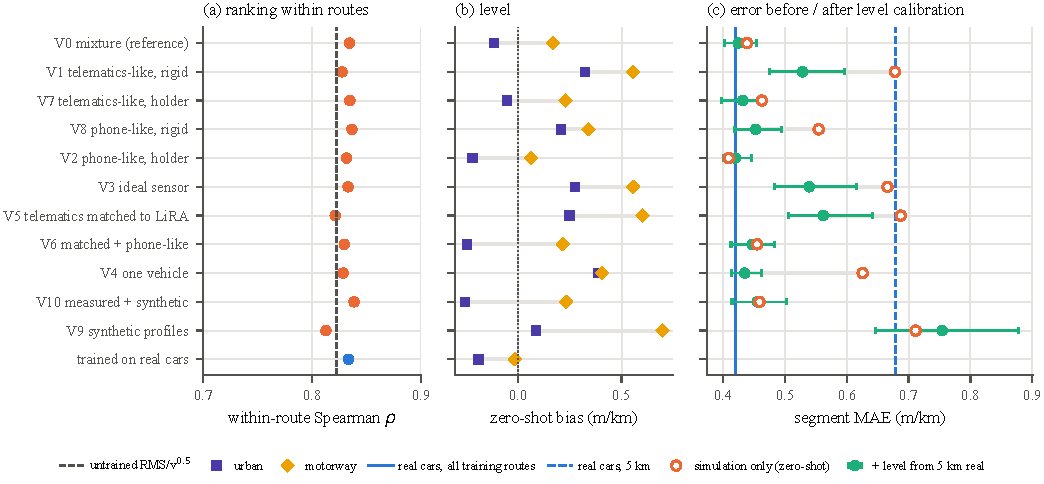
\includegraphics[width=\textwidth]{v2_variants.pdf}
\caption{Simulator variants, LightGBM trained on simulated drives only and tested on the held-out real routes. (a) Within-route Spearman $\rho$ (real-trained model in blue; dashed: the untrained statistic RMS$/v^{0.5}$). (b) Zero-shot bias on urban and motorway segments. (c) Pooled segment MAE zero-shot (open circles) and after a level offset estimated from 5\,km of real passes of the training routes (filled; bars: 2.5--97.5\,\% range over 20 draws); solid line: trained on all real training data; dashed: trained on 5\,km of real data.}
\label{fig:variants}
\end{figure*}

V0's agreement in level is not a robust property of simulating over measured profiles (Table~\ref{tab:variants}, Fig.~\ref{fig:variants}).
Across the nine variants on measured profiles (V0--V8), the within-route $\rho$ stays between \vvRhoMin{} and \vvRhoMax, the partial $\rho$ between \vvPrhoMin{} and \vvPrhoMax{} and the scale $b$ between \vvScaleMin{} and \vvScaleMax{} (real-trained: \vvRealScaleB), whereas the pooled zero-shot bias ranges from \vvBiasMin{} to \vvBiasMax\,m/km and the MAE from \vvMaeMin{} to \vvMaeMax.
The 2$\times$2 sensor design shows what set V0's level: adding the holder resonance changes the bias by \vvHolderEffTele\,m/km for the telematics-like and by \vvHolderEffPhone\,m/km for the phone-like sensor, switching the sensor family by \vvFamilyEffRigid{} (rigid) and \vvFamilyEffHolder\,m/km (with holder).
V0 thus owes its level mainly to the holder resonance of its phone-like half, a component meant to model phone holders rather than the car's telematics unit.
An ideal sensor (V3) and a telematics sensor matched to the rates, quantisation, noise and tilt measured on the LiRA-CD streams (V5) both overestimate by about 0.4\,m/km, and so does a single mid-range vehicle (V4).
Synthetic profiles alone (V9) still rank segments ($\rho=$\,\vvVnineRhoWithin) but overestimate on motorways (bias \vvVnineBiasMotorway\,m/km); adding them to the measured profiles (V10) changes little.
The earlier game-engine corpus does not transfer under this protocol (within-route $\rho=$\,\vvBcorrRhoWithin, MAE \vvBcorrMae\,m/km; Supplement~\ref{S-sec:s_earlier}).

\begin{figure*}[t]
\centering
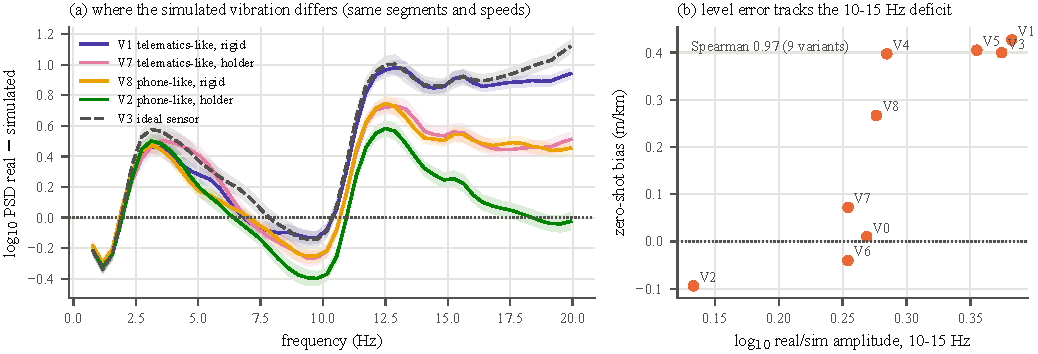
\includegraphics[width=\textwidth]{v2_spectra.pdf}
\caption{(a) Mean difference of log$_{10}$ power spectral density, real minus simulated, on the same segments in the same 10\,km/h speed bands (re-simulated passes of four sensor variants and the ideal sensor; bands: 95\,\% intervals from a 1\,km-block bootstrap). (b) Zero-shot bias of the nine measured-profile variants against the real/simulated amplitude ratio of the 10--15\,Hz band (log$_{10}$).}
\label{fig:spectra}
\end{figure*}

\subsection{Where the simulated vibration differs}
\label{sec:res_mech}

On the same segments and speed bands, the real car's vibration differs from all simulated variants in the same way below 10\,Hz and differently above (Fig.~\ref{fig:spectra}a, Table~\ref{S-tab:s_spectra}): all variants lack energy at 2--5\,Hz (real/simulated power \spVoneMidPow--\spVfiveMidPow) and match it at 5--10\,Hz, whereas at 10--15\,Hz the real car has \spVthreeHighPow{} and \spVoneHighPow{} times the power of the ideal and the rigid telematics-like sensor but only \spVtwoHighPow{} times that of the phone-like sensor with holder resonance.
Across the nine variants the zero-shot bias orders like this 10--15\,Hz deficit (Spearman \bgRhoHigh; Fig.~\ref{fig:spectra}b), as expected if an estimator trained on too little simulated vibration reads the car's extra vibration as roughness, not like the deficits at 0.5--2 or 2--5\,Hz (\bgRhoLow{} and \bgRhoMid), and the deficit is larger on motorway than on urban segments for \bgcMotorwayLarger{} of \bgcNvar{} variants (amplitude ratio \bgcMotorwayMin--\bgcMotorwayMax{} vs \bgcUrbanMin--\bgcUrbanMax; Table~\ref{S-tab:s_gap}), as is the bias.
The real car's empirical transmissibility peaks at \invPeakHz\,Hz (Fig.~\ref{S-fig:s_acf}b).
Passes logged at 333\,Hz contain more, not less, 10--15\,Hz power than passes logged at 52.6\,Hz on the same cells (\spAliasHigh{} in log$_{10}$, confounded with the device), so the excess is not an aliasing artefact of the slower logging; its physical source is not identified (the half-car has no roll or body flexibility, and the mounting of the telematics unit and the unsprung dynamics of the car are unknown).

A second mismatch is common to all variants: on a fixed road the real car's vibration RMS rises with speed with elasticity \ssRealUrban{} [\ssRealUrbanLo, \ssRealUrbanHi] on urban and \ssRealMotorway{} [\ssRealMotorwayLo, \ssRealMotorwayHi] on motorway segments, the simulated vibration over the same segments at the same speeds with \ssSimUrbanMin--\ssSimUrbanMax{} and \ssSimMotorwayMin--\ssSimMotorwayMax{} (Table~\ref{S-tab:s_gap}).
The simulator does not reproduce how the car's vibration scales with speed; as this mismatch is similar for all variants, it does not explain their different levels.

\subsection{How much paired real data is needed}
\label{sec:res_value}

Fig.~\ref{fig:value} and Table~\ref{tab:value} compare simulation with paired real drives on the same 20 draws of $k$\,km of training-route road; Table~\ref{S-tab:s_value_variants} gives every variant.
Two real-only comparators are used, LightGBM and the three-parameter vibration index, which suits very small samples better (\vbRealIdxOne{} vs \vbRealOnlyOne\,m/km at 1\,km).
The ranges over draws reflect which $k$\,km are drawn, not the uncertainty of the test routes.

\begin{figure*}[t]
\centering
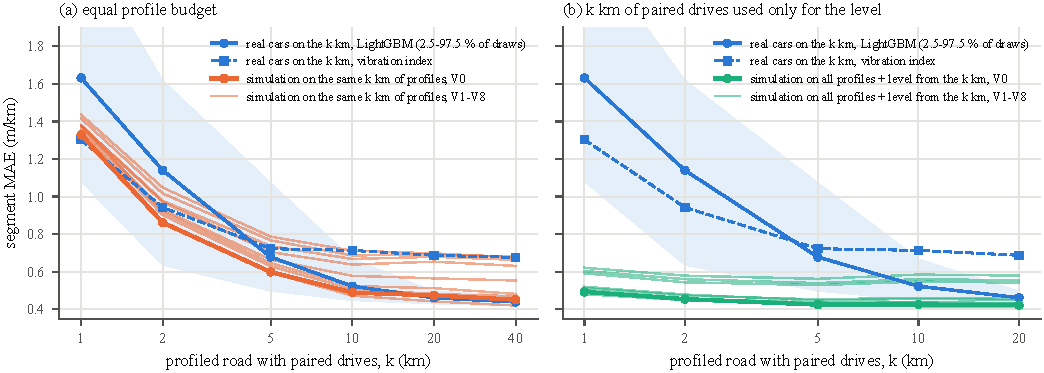
\includegraphics[width=\textwidth]{v2_value.pdf}
\caption{Simulation against paired real drives on the same 20 draws of $k$\,km of training-route road (pooled segment MAE on the held-out routes). Blue: trained on the real passes over the $k$\,km, LightGBM (band: 2.5--97.5\,\% of draws, clipped at the top) or the three-parameter vibration index (dashed). (a) Equal profile budget: LightGBM trained on simulated passes over the profiles of the same $k$\,km (bold: V0; thin: V1--V8). (b) LightGBM trained on simulated passes over all training-route profiles, with a level offset estimated from the real passes over the $k$\,km.}
\label{fig:value}
\end{figure*}

% AUTO-GENERATED by research_rescue/make_tables_v2.py from results/v2 - do not edit by hand.
\begin{table}[t]
\centering
\caption{Simulation against paired real drives on the same 20 draws of $k$\,km of training-route road (pooled segment MAE in m/km on the held-out routes; brackets: 2.5--97.5\,\% of draws). Real-only: LightGBM or the three-parameter vibration index trained on the real passes over the $k$\,km. Same $k$\,km: LightGBM trained on V0 simulated passes over the profiles of the same $k$\,km, with the paired difference to real-only LightGBM and the number of the 20 draws in which simulation was better. All + level: LightGBM trained on simulated passes over all training-route profiles with a level offset from the $k$\,km of real passes, range of the means over the nine measured-profile variants V0--V8.}
\label{tab:value}
\setlength{\tabcolsep}{2pt}
\scriptsize
\begin{tabular}{@{}rcccccc@{}}
\toprule
& \multicolumn{2}{c}{Real-only} & \multicolumn{3}{c}{Same $k$\,km, simulated (V0)} & All + level \\ \cmidrule(lr){2-3}\cmidrule(lr){4-6}
$k$ & LightGBM & index & MAE & $-$ real & better & V0--V8 \\
\midrule
1 & 1.63 [1.08, 2.36] & 1.30 & 1.33 & $-$0.30 & 20 & 0.48--0.62 \\
2 & 1.14 [0.63, 1.62] & 0.94 & 0.86 & $-$0.28 & 20 & 0.45--0.58 \\
5 & 0.68 [0.50, 1.07] & 0.72 & 0.60 & $-$0.08 & 16 & 0.42--0.56 \\
10 & 0.52 [0.45, 0.67] & 0.71 & 0.49 & $-$0.03 & 15 & 0.42--0.58 \\
20 & 0.46 [0.43, 0.50] & 0.69 & 0.47 & +0.01 & 9 & 0.41--0.58 \\
40 & 0.44 [0.42, 0.47] & 0.68 & 0.45 & +0.01 & 3 & -- \\
\midrule
all & 0.42 & -- & 0.44 & -- & -- & -- \\
\bottomrule
\end{tabular}
\end{table}


\emph{Equal profile budget} (Fig.~\ref{fig:value}a).
Simulated drives over the profiles of the $k$\,km are not a general substitute for the real drives over them.
With 1--2\,km, simulated LightGBM beats real-trained LightGBM for every variant but not the real-trained index (simulation better in \pcSameWinsIdxOneMin--\pcSameWinsIdxOneMax{} of 20 draws at 1\,km), and all these errors exceed \pcSameMaeTwoMin\,m/km.
From 5\,km on the answer depends on the simulator: at 20\,km the difference to real-only LightGBM ranges from \pcSameDiffTwentyMin{} to \pcSameDiffTwentyMax\,m/km over the nine variants, small for V0 and V2 (\pcSameVzeroDiffTwenty{} and \pcSameVtwoDiffTwenty) and largest for V1, V3 and V5, the variants with the largest 10--15\,Hz deficit (\pcSameHiDefDiffTwentyMin--\pcSameHiDefDiffTwentyMax).
A level offset from the same $k$\,km closes the gap of the single-vehicle variant V4 (\pcSameCalVfourDiffTwenty\,m/km at 20\,km) but not that of these three.

\emph{Paired drives used only for the level} (Fig.~\ref{fig:value}b).
Trained on simulated drives over all profiled training roads and calibrated with a level offset from 5\,km of paired drives, every variant reaches \pcCalMaeFiveMin--\pcCalMaeFiveMax\,m/km, better than real-only LightGBM on those 5\,km (\vbRealOnlyFive\,m/km) in \pcCalWinsFiveMin--\pcCalWinsFiveMax{} of 20 draws and better than the real-only index (\vbRealIdxFive\,m/km) in \pcCalWinsIdxFiveMin--\pcCalWinsIdxFiveMax; real training on all data of the training routes reaches \vrGbmMae\,m/km, the six variants other than V1, V3 and V5 \pcCalLoDefMaeFiveMin--\pcCalLoDefMaeFiveMax\,m/km.
The advantage at 5\,km holds on each held-out route for every variant (mean difference per route \pcRouteFiveDiffMin{} to \pcRouteFiveDiffMax\,m/km).
With more paired data, real-only LightGBM overtakes V1, V3 and V5: the calibrated simulation is better in only \pcCalHiDefWinsTenMin--\pcCalHiDefWinsTenMax{} of 20 draws at 10\,km and in none at 20\,km, while for the other six variants it is still better in \pcCalLoDefWinsTwentyMin--\pcCalLoDefWinsTwentyMax{} of 20 draws at 20\,km.
For these three variants a level offset is not enough; an affine calibration from 20\,km brings them to \pcAffHiDefMaeTwentyMin--\pcAffHiDefMaeTwentyMax\,m/km.
Simulation over all profiled roads plus a level from a few kilometres of paired drives was thus the most data-efficient option for every variant; how long it stays ahead of real drives depends on how closely the simulated vibration matches the car's.

\begin{figure}[t]
\centering
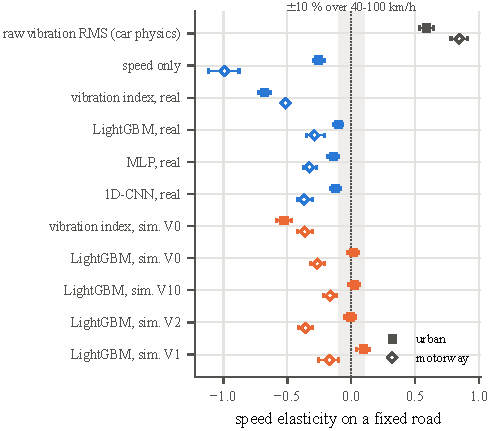
\includegraphics[width=\columnwidth]{v2_speed.pdf}
\caption{Speed elasticity of each estimate on a fixed real road (slope of log estimate on log speed with segment fixed effects; 95\,\% intervals from a 1\,km-block bootstrap; urban and motorway segments). Grey band: $\pm$10\,\% change between 40 and 100\,km/h. Top row: raw vibration RMS of the real car.}
\label{fig:speed}
\end{figure}

% AUTO-GENERATED by research_rescue/make_tables_v2.py from results/v2 - do not edit by hand.
\begin{table*}[t]
\centering
\caption{Controlled simulation (class S; no real data). Left: number of training vehicles at a fixed 1,200 training passes (held-out synthetic routes, 30 unseen and up to 30 seen vehicles; LightGBM). $\Delta$: unseen minus seen MAE relative to seen, with the upper 95\,\% bound from a segment and from a route bootstrap; criterion of our earlier study: upper bound $\le$10\,\%. Right: one sensor property changed at test time (LightGBM trained on synthetic profiles with the sensor mixture, tested on 12 held-out synthetic routes driven by 6 unseen vehicles with the telematics-like sensor; MAE and bias in m/km).}
\label{tab:general}
\setlength{\tabcolsep}{3pt}
\footnotesize
\begin{tabular}[t]{@{}rccccc@{}}
\toprule
Vehicles & Seen & Unseen & $\Delta$ & Upper bound (\%) & Criterion met \\
$N$ & MAE & MAE & (\%) & segments / routes & segments / routes \\
\midrule
3 & 0.62 & 1.06 & $+$70 & 76 / 87 & no / no \\
10 & 0.75 & 0.92 & $+$24 & 27 / 31 & no / no \\
30 & 0.78 & 0.90 & $+$16 & 18 / 21 & no / no \\
100 & 0.82 & 0.87 & $+$6 & 8 / 11 & yes / no \\
300 & 0.81 & 0.87 & $+$7 & 9 / 12 & yes / no \\
\bottomrule
\end{tabular}\hspace{6mm}
\begin{tabular}[t]{@{}lcc@{}}
\toprule
Sensor property at test time & MAE & Bias \\
\midrule
telematics-like, rigid (reference) & 0.84 & $-$0.65 \\
+ holder resonance 40 Hz & 0.79 & $-$0.55 \\
+ holder resonance 25 Hz & 0.73 & $-$0.36 \\
+ holder resonance 15 Hz & 0.88 & +0.37 \\
sampling rate 200 Hz & 0.77 & $-$0.48 \\
sampling rate 50 Hz & 0.87 & $-$0.71 \\
sampling rate 25 Hz & 1.39 & $-$1.36 \\
speed error $+$20\,\% & 1.06 & $-$0.98 \\
speed error $-$20\,\% & 0.73 & $-$0.15 \\
white noise $\times$8 & 0.82 & $-$0.58 \\
mounting tilt s.d.\ 20$^\circ$ & 0.84 & $-$0.64 \\
40\,\% samples lost & 0.94 & $-$0.81 \\
\bottomrule
\end{tabular}
\end{table*}


\subsection{Speed dependence on a fixed road}
\label{sec:res_speed}

Each segment was driven about ten times at different speeds (median within-segment SD of log speed \elSdLogv), so the speed dependence of every estimate can be measured on a road of constant roughness (Fig.~\ref{fig:speed}, Table~\ref{S-tab:s_speed}).
The real car's vibration RMS rises by \elRawPooledPct\,\% between 40 and 100\,km/h (elasticity \elRawPooled{} [\elRawPooledLo, \elRawPooledHi]).
The learned estimators and the vibration index trained on real cars over-correct for it: LightGBM's estimate falls by \elRealGbmPooledPct\,\% over the same range (\elRealGbmPooled{} [\elRealGbmPooledLo, \elRealGbmPooledHi]), and without speed inputs it still falls (\elRealGbmNoSpeedPooled); the MLP and CNN behave alike (\elRealMlpPooled{} and \elRealCnnPooled) and the vibration index over-corrects most (\elRealIdxPooled).
Simulation-trained LightGBM V0 changes by \elSimGbmPooledPct\,\% (\elSimGbmPooled{} [\elSimGbmPooledLo, \elSimGbmPooledHi]).
Paired on the same passes, its elasticity exceeds that of the real-trained model by \epVzeroPooled{} [\epVzeroPooledLo, \epVzeroPooledHi] (5\,km blocks), entirely on urban roads (\epVzeroUrban{} [\epVzeroUrbanLo, \epVzeroUrbanHi]; motorways \epVzeroMotorway{} [\epVzeroMotorwayLo, \epVzeroMotorwayHi]).
Across the nine variants the pooled elasticity ranges from \elSimGbmMeasPooledMin{} to \elSimGbmMeasPooledMax{} (\elSimGbmMeasInside{} of 9 inside the $\pm$10\,\% band), the paired difference from \epMeasPooledMin{} to \epMeasPooledMax{} (interval excluding zero for \epMeasPooledExcl{} of 9); on motorways every estimate falls with speed (simulation-trained \elSimGbmMeasMotorwayMin{} to \elSimGbmMeasMotorwayMax, real-trained \elRealGbmMotorway).
Simulation thus removes part of the over-correction that real-trained estimators show on urban roads, but it does not make estimates speed-invariant, and the simulation-trained vibration index still over-corrects strongly (\elSimIdxPooled).
Given the speed-scaling mismatch of Section~\ref{sec:res_mech}, this is a property of the learned estimators, not evidence that the simulator reproduces the car's speed response.

\subsection{Other vehicles and sensors: simulation only}
\label{sec:res_vehicles}
LiRA-CD contains one car model, so transfer to other vehicles can be examined only in simulation (class S, Table~\ref{tab:general}, Fig.~\ref{fig:vehicles}).
With the amount of training data fixed at 1,200 passes, the MAE on 30 unseen vehicles exceeds that on the training vehicles by \vsThreeRel\,\% with 3 training vehicles, \vsThirtyRel\,\% with 30 (the number used in V0) and \vsHundredRel\,\% with 100.
The criterion of our earlier study (upper bound $\le$10\,\%) is met from 100 vehicles with a segment bootstrap but not with a route bootstrap (upper bounds \vsHundredRelHiRoute{} and \vsThreeHundredRelHiRoute\,\% for 100 and 300 vehicles).
The gap closes from both sides: the error on unseen vehicles falls (\vsThreeUnseen{} to \vsHundredUnseen\,m/km from 3 to 100 vehicles) and the error on training vehicles rises as each gets fewer passes (\vsThreeSeen{} to \vsHundredSeen\,m/km).
At $N=30$, a vehicle's error is only weakly related to its parameter distance from the nearest training vehicle (Spearman \vsDistRho{} over 30 vehicles).

\begin{figure}[t]
\centering
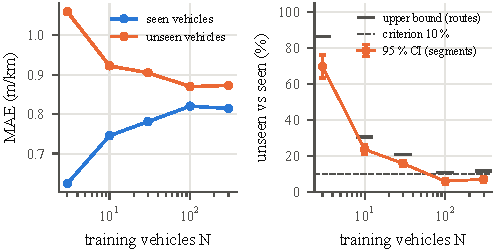
\includegraphics[width=\columnwidth]{v2_vehicles.pdf}
\caption{Number of training vehicles at a fixed 1,200 training passes (simulation only). Left: MAE on seen and unseen vehicles. Right: relative increase from seen to unseen vehicles with 95\,\% interval (segment bootstrap) and the upper bound of a route bootstrap; dashed: 10\,\% criterion.}
\label{fig:vehicles}
\end{figure}

Sensor perturbations at test time (Table~\ref{tab:general}, bottom) reproduce in simulation what the variants showed on the real car: the sensor path moves the level.
A holder resonance at 15\,Hz turns a bias of \rbvGbmBiasMountRigid{} into \rbvGbmBiasMountFifteen\,m/km; 25\,Hz sampling and a speed error of $+$20\,\% are the most harmful perturbations (MAE \rbvGbmMaeRateTwentyFive{} and \rbvGbmMaeSpeedPlus\,m/km), white noise, tilt and lost samples the least.
